
The RoboTutor system architecture consists of several components. The overall design has been based mainly on some practical considerations related to being able to present and manipulate a slideshow and to perform associated interactive behaviours on the robot itself.  The main components for handling a slideshow (we have used PowerPoint \cite{PowerPoint} and TurningPoint \cite{TurningPoint}) are run on a laptop computer whereas other interaction behaviours are run on the Nao itself. Fig. \ref{fig:system_overview} provides an overview of these components; in the figure, red arrows represent control flow and black arrows represent data flow. The robot and laptop computer communicate with each other through a protocol called Google Protocol Buffers \cite{protobuf}. Google Protocol Buffers provide a language- and platform-neutral tool that is easily extended and used by the RoboTutor system to exchange a script or commands between the laptop computer and the robot over a network channel.

\begin{figure}
\centering
	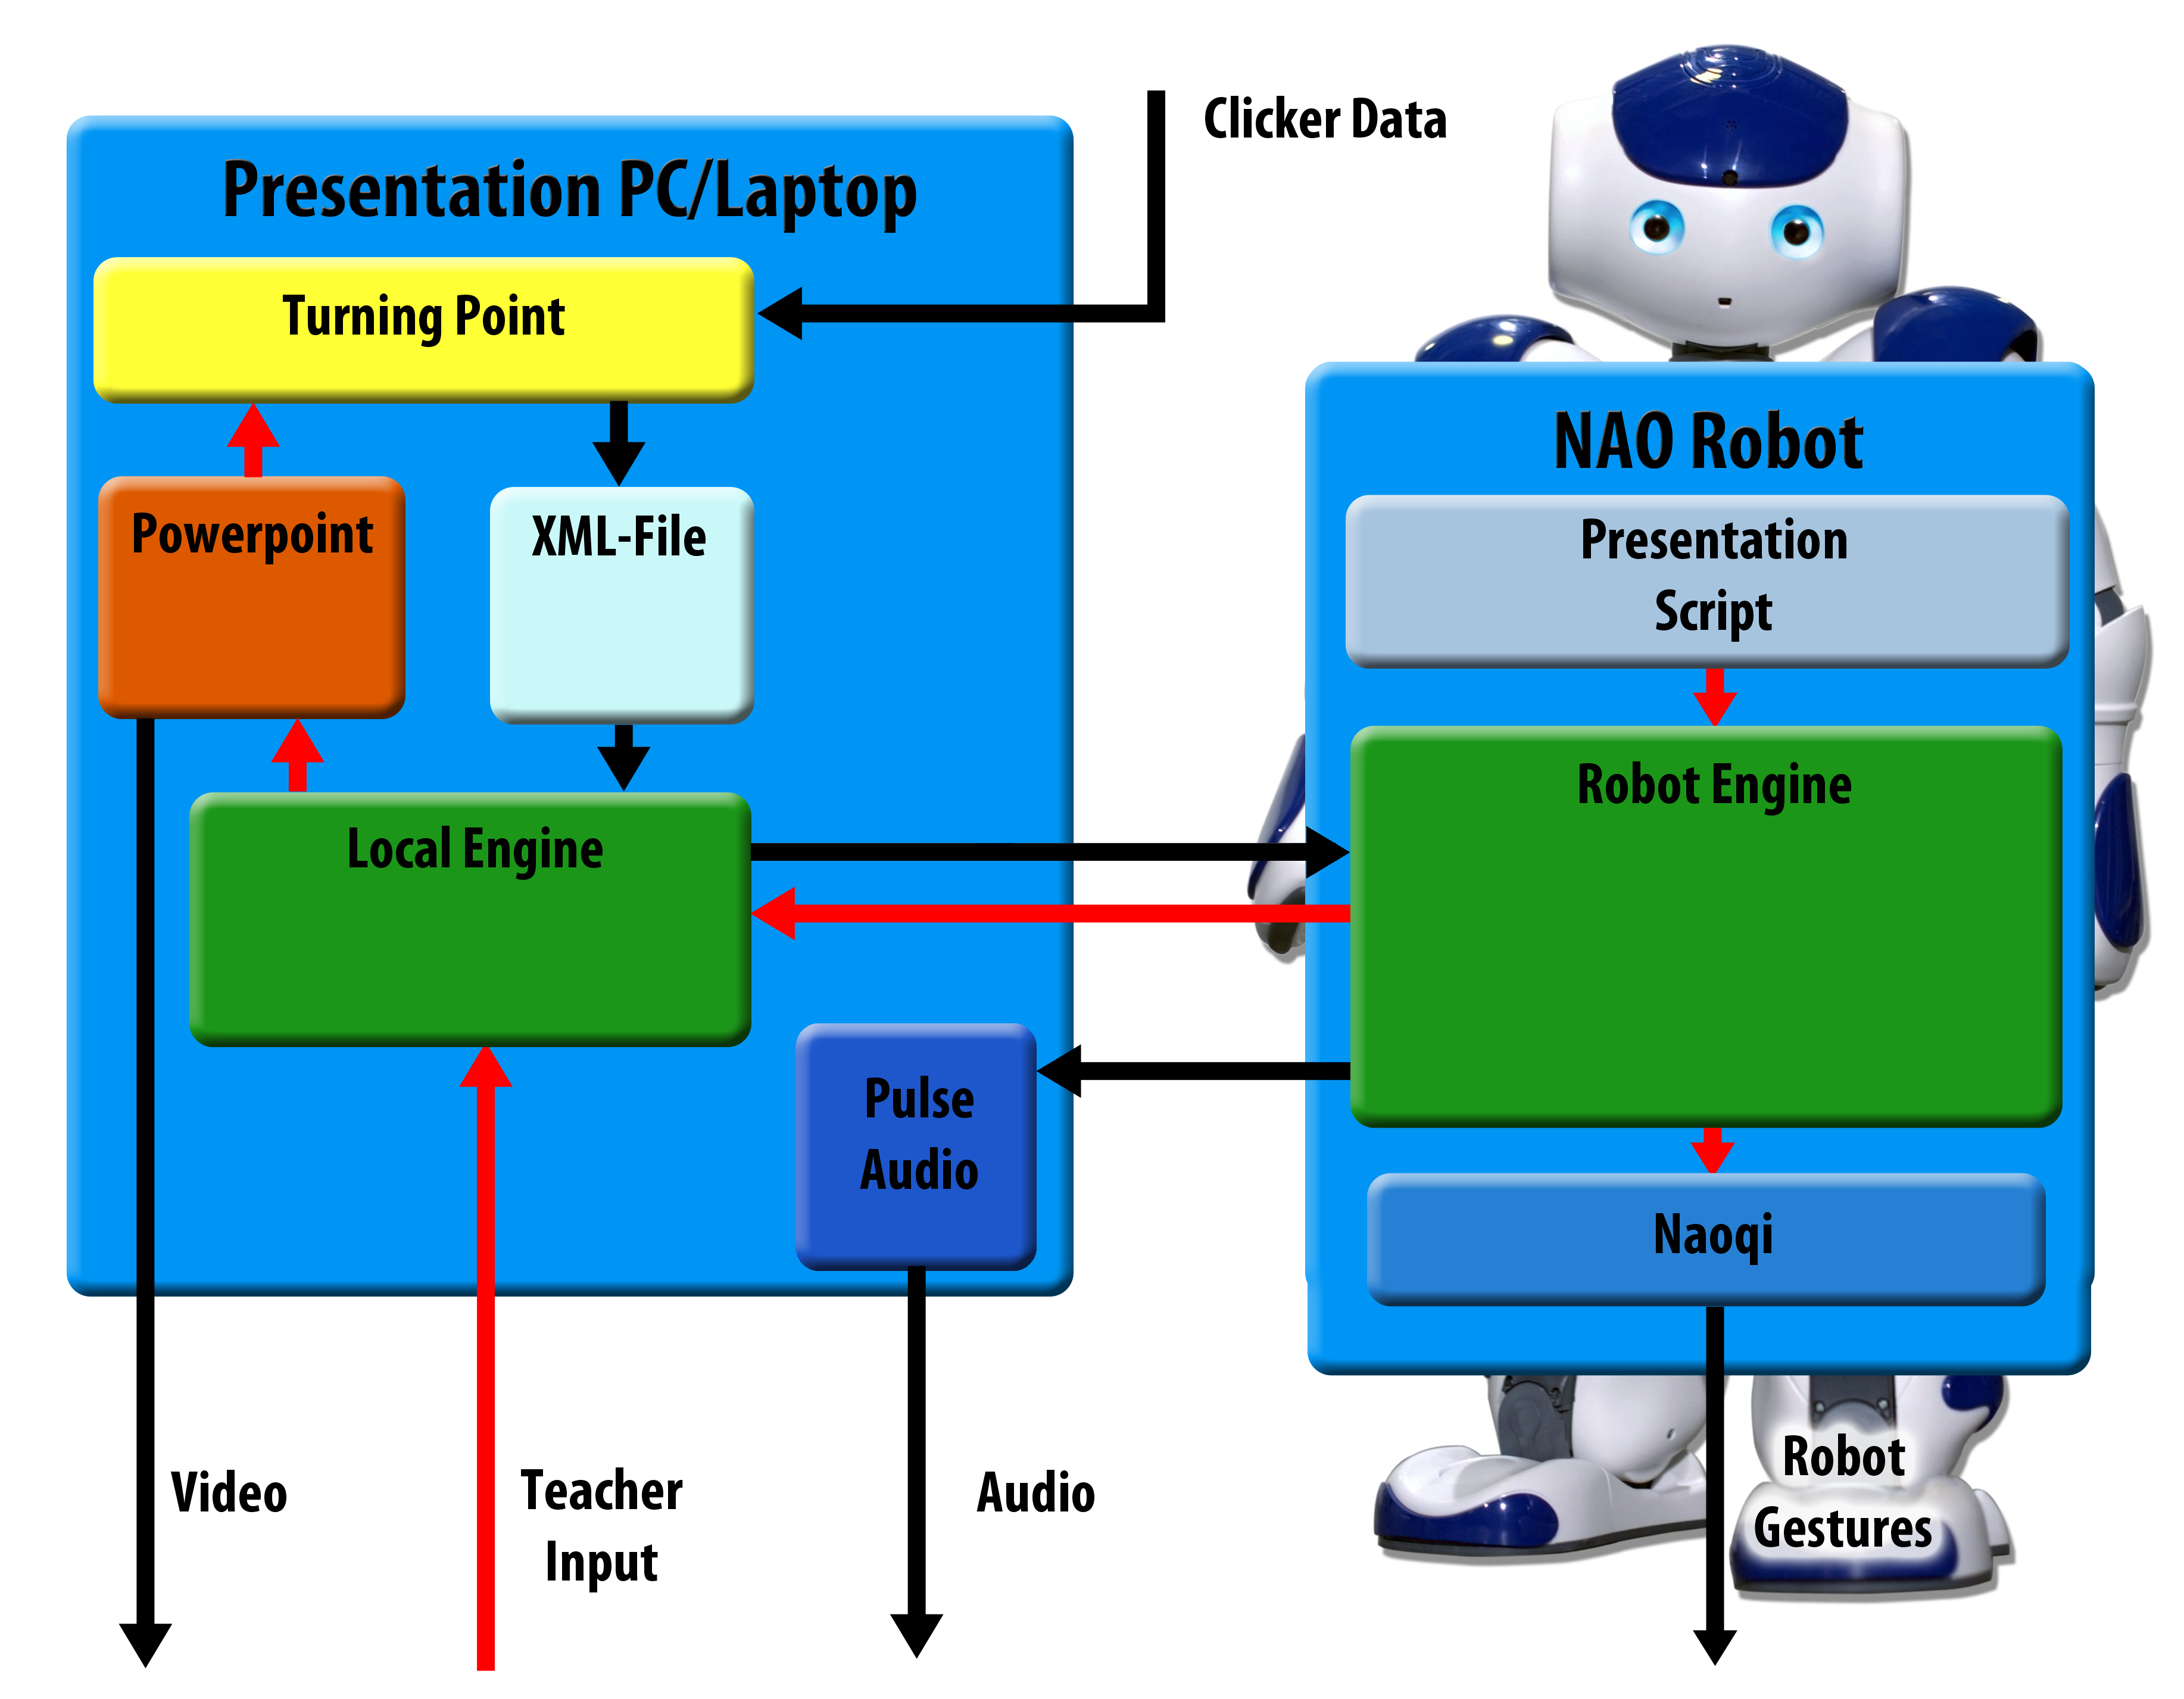
\includegraphics[scale=0.07]{images/system_overview.png}
	\caption{Overview of the RoboTutor System}\label{fig:system_overview}
\end{figure}

%
\paragraph{Script Engine and Editor}
The RoboTutor uses a script engine that runs on the Nao to present a lecture. A script consists of a series of commands, including the possibility to branch depending on input received during the presentation, changing slides in a slideshow and performing arbitrary behaviours that the Nao is capable of. An important part of a script is to control the ``body language" of the robot (e.g., gestures) to support the text spoken by the Nao. Currently, supported behaviours include various behaviours for moving the arm, legs and head together or separately as a (human) presenter would (e.g., for performing a pointing behaviour). Additional and more complex behaviours such as dance behaviours are easily integrated by means of Choregraphe. %\cite{choregraphe}.
 Other commands that are available include taking a picture of the audience, controlling the pace of the slideshow and pausing/resuming the execution of the script. Moreover, at any moment a human (teacher) can pause and resume the execution of the script using the script GUI or by touching the head of the Nao.

A simple GUI that can be launched on the laptop computer contains a text editor that can be used to create a script. %This editor has basic syntax highlighting capabilities (to differentiate, e.g., spoken text from behaviour commands and comments).
When the script is run, it is sent to the script engine on the robot. A custom script parser has been written in C++ which executes the script in real time. Plain text in the script is sent to the speech engine running on the Nao and the commands are being handled separately. In case a command to run a behaviour is received, it is added to a queue and is executed when the speech engine notifies it is time for that behaviour to be executed. Currently, synchronising text and behaviours of the Nao is done by letting the Nao perform a behaviour that matches the context of the text and the duration of the spoken text. Commands to change a slide are sent back to the laptop computer which forwards these to PowerPoint.

%
\paragraph{Presentation Application}
The laptop computer is connected to a beamer and is used to project the slideshow on a screen. The main component executed on the laptop used for presenting the slideshow is an engine that is created using the Qt-toolkit \cite{QT}. Qt is a graphical toolkit written in C++ that is commonly used for cross platform applications and supports the development of user interfaces. By means of the Qt user interface the user has control over the RoboTutor application code that runs on the robot itself. It facilitates connecting to the robot, and allows controlling the script by either pausing, running, or terminating a script. By launching the interface, PowerPoint is also automatically launched and a communication link between the engine and PowerPoint is created. This allows the laptop application to control the PowerPoint slideshow and trigger, e.g., a next slide event for moving to the next slide. The RoboTutor can move to the next slide, step back or forward an arbitrary number of slides, or go to a specific slide. It is even possible to dynamically create and add a slide to the slideshow while the robot is giving a presentation. One use case for this feature is to take a picture using one of Nao's cameras and display it on a newly created slide. This usually means the audience can see itself, creating a humorous moment; it, moreover, also to some extend suggests that the robot is aware of its audience.

%
\paragraph{Support for Quizzes}
The TurningPoint system consists of a number of response cards (small electronic devices) connected to a computer. These response cards are handed out to participants in the audience. The cards can be used to (digitally) indicate a choice in reply to a multiple-choice question that is projected on a slide. The results are received and aggregated by the TurningPoint. The TurningPoint software is an integral part of the RoboTutor system and enables the RoboTutor to ask questions and interpret the results. This in turn enables the RoboTutor to react and respond to audience input. The RoboTutor can also use this tool to decide on how to proceed in a lecture. For example, the robot can ask whether a concept is clear to the audience or more explanation is needed. Based on feedback from the audience, the robot can make a decision on how to proceed.

TurningPoint questions are started by a command in the script. The script engine running on the robot then requests the local engine to initiate a TurningPoint session through Powerpoint. After TurningPoint has polled the answers from the audience, the local engine component receives and processes an XML-file that contains the results of the quiz. These are then sent to the robot's script engine, which upon receiving the results makes a decision on what to do next.

%
\paragraph{Audio} The laptop computer can also be connected to an audio system if that is available in a classroom to route and enhance audio output of the Nao. In large rooms or lecture halls, the maximum volume of Nao's internal speakers may not be sufficient to enable the audience to follow the lecture properly. To handle these situations audio streaming has been enabled in the Nao. Using pulse audio, the Nao's sound can be redirected to a different set of speakers. 
The RoboTutor is also able to monitor the noise level in the room, and respond accordingly if there is too much noise. Additionally the noise level can be visualized live on a PowerPoint slide.
